\documentclass[a4paper,12pt]{article}
\usepackage{amsmath}
\usepackage{amssymb}
\usepackage{graphicx}
%\documentclass{article}
\usepackage{setspace, enumitem,titlesec}
\usepackage{calc}
			% Activate to display a given date or no date
\usepackage{mathtools}
\usepackage{mathrsfs }
\DeclarePairedDelimiter\ceil{\lceil}{\rceil}
\DeclarePairedDelimiter\floor{\lfloor}{\rfloor}
\usepackage{algorithm}
\usepackage{algorithmic}
\usepackage{fancybox}

\usepackage{amsmath}
\usepackage{amssymb}
\usepackage{amsthm}
\usepackage{cite}
%\usepackage{algpseudocode}
\begin{document}
%\renewcommand{\thepseudonum}{\roman{pseudonum}}
\renewcommand\labelenumi{(\theenumi)}
%vector
\renewcommand{\vec}[1]{\mathbf{#1}}
\title {Review of Week 3 }
%\author{jim.morris.shen@gmail.com}
%\author{The Graduate Center, City University of New York}
\author{Xiaoke(Jimmy) Shen}
%\author{The Graduate Center, City University of New York}
\maketitle
%\textbf{Due Mar 1st 11:59 pm. 10 points for each exercise and 20 points for the extra credit exercise }\\
\section{Introduction}

This paper review report is provided based on the requirement of the computer science research course provided by the Graduate Center of the City University of New York during the 2017 Fall Semester. The main objective of this course is helping the PHD candidates to prepare their second exam and identify their thesis topic as early as possible\cite{ji2017}. \\

\section{Object Classification for 2D Images}
\subsection{ImageNet Classification with Deep Convolutional Neural Networks\cite{NIPS2012_4824}}
In the ILSVRC-2012 competition and achieved a winning top-5 test error rate of $15.3\%$, compared to $26.2\%$ achieved by the second-best entry\cite{NIPS2012_4824}. The outstanding performance of the deep neural network used in this paper brought the focus of both the academic and industry back to the neural network again. In this paper, the CNN network is used and the CNN network structure is illustrated in the Figure \ref{fig:alexnet}. Two GPUs were used to speed up the calculation. Dropout \cite{DBLP:journals/corr/abs-1207-0580} was used here and was proved to be effective to reduce the overfitting problem. The cons of this network is it is a bit complicated and the structure is not so elegant and it will be addressed in the future works by the deep learning researchers.

 \begin{figure}[H]
  \begin{center}
      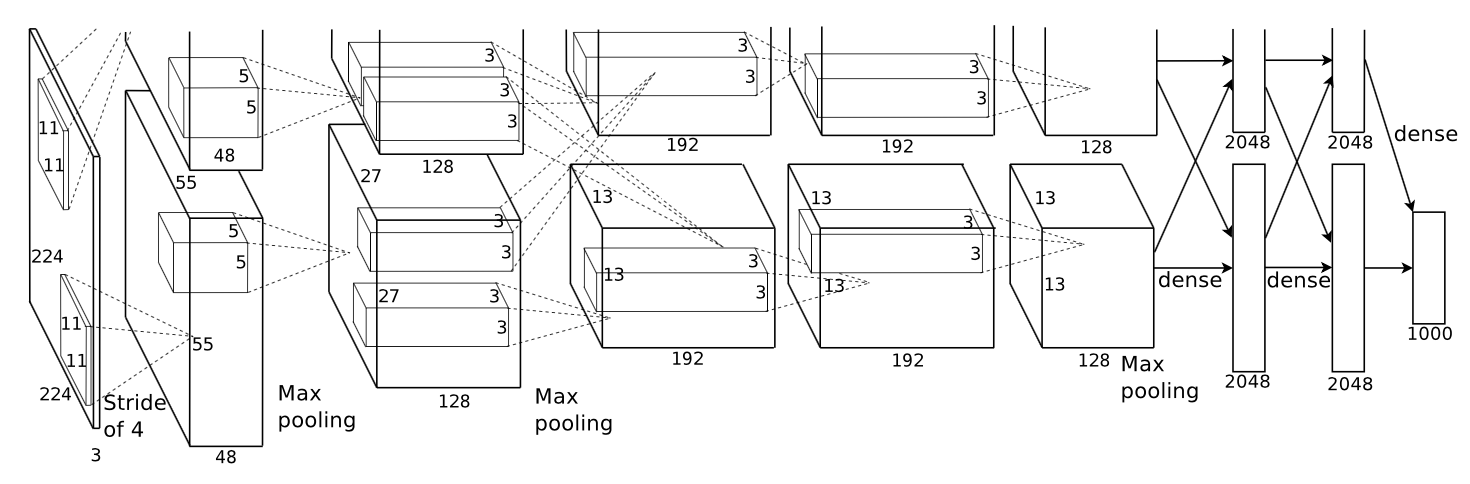
\includegraphics[scale=0.55]{alexnet.png}
\end{center}
\caption{An illustration of the architecture of Alex Net, explicitly showing the delineation of responsibilities between the two GPUs. One GPU runs the layer-parts at the top of the figure while the other runs the layer-parts at the bottom. The GPUs communicate only at certain layers. The network?s input is 150,528-dimensional, and the number of neurons in the network?s remaining layers is given by 253, 440-186, 624-64, 896-64, 896-43, 264-4096-4096-1000\cite{NIPS2012_4824}.}
 \label{fig:alexnet}
 \end{figure}

\subsection{Very Deep Convolutional Networks for Large-Scale Image Recognition\cite{SimonyanZ14a}}
One important contribution of the VGG network is the structure of this network is very tidy and elegant. Different to the Alex  Net\cite{NIPS2012_4824} with different size of the convolutional kernels, in the VGG CNN network\cite{SimonyanZ14a} , only size of 3 by 3 kernels were used for the whole network. At the same time, the trained network weights based on the ImageNet\cite{imagenet_cvpr09} dataset were shared to public. The cons of this model is there are too many parameters and the computation took a long time. Weeks for doing the ImageNet\cite{imagenet_cvpr09}  dataset by using a powerful GPU. \\
This elegant design can also be used in the 3D CNN network to address the 3D object classification problem which is my current working topic.\\
 \begin{figure}[H]
  \begin{center}
      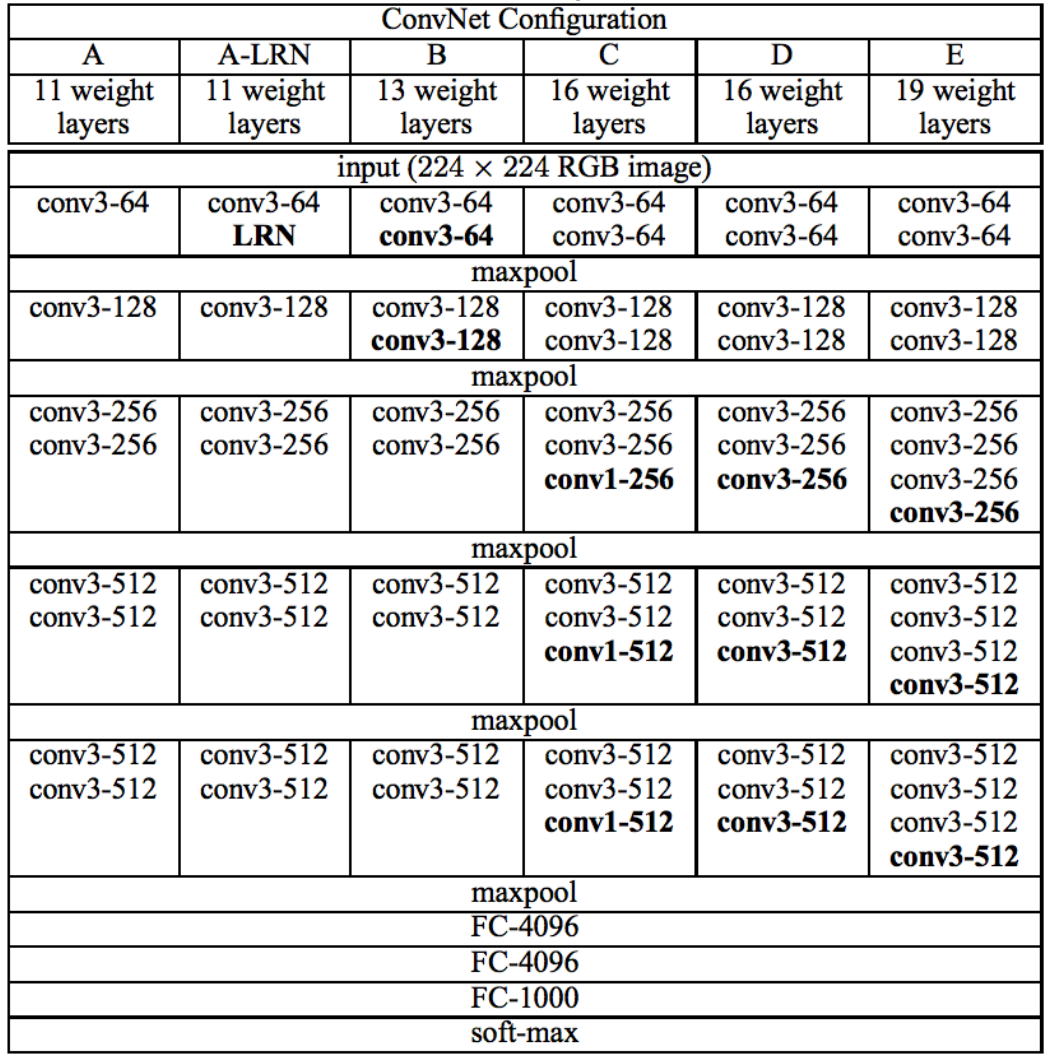
\includegraphics[scale=0.75]{vgg16.png}
\end{center}
\caption{An illustration of the VGG network structure.}
 \label{fig:vgg16}
 \end{figure}

\subsection{Deep Residual Learning for Image Recognition\cite{DBLP:journals/corr/HeZRS15}}
In motivation of this work is trying to find a deeper neural network structure to achieve better performance as the deepest network prior this work is around 20 to 30 layers. The authors had a basic assumption that if more layers are added, the performance should be at least the same as the less layer networks as the new added layers can be designed as the identify layer then the performance can be at least the same. However, the traditional network's performance decreases when the layers increases to a higher level as shown in Figure \ref{fig:resnet}. In order to address this anti-intuitive problem, the authors of this paper designed a deep residual network by adding a short cut between every other layers and finally it shows that this network can achieve a better performance. The problem is addressed. In this paper, the layer of the neural network can goes to 110 layer and have a better performance than the previous state-of-the-art neural network such as VGG16\cite{SimonyanZ14a}, which only has 16 layers neural network. However, as mentioned in \cite{DBLP:journals/corr/HeZRS15}, the parameters used for the 110 layers Resnet is even less than the 16 layers VGG16 network. This seems amazing. However, by reading this article carefully, the main contribution of the reduction of the parameters was using the convolutional network layer instead of the fully connected layer. There is no contribution on the parameters reduction by the Resnet itself.\\

Of course, the Resnet structure used for the 2D images can be further studied to see whether can also be used for the 3D cloud point data.\\ 
\begin{figure}[H]
  \begin{center}
      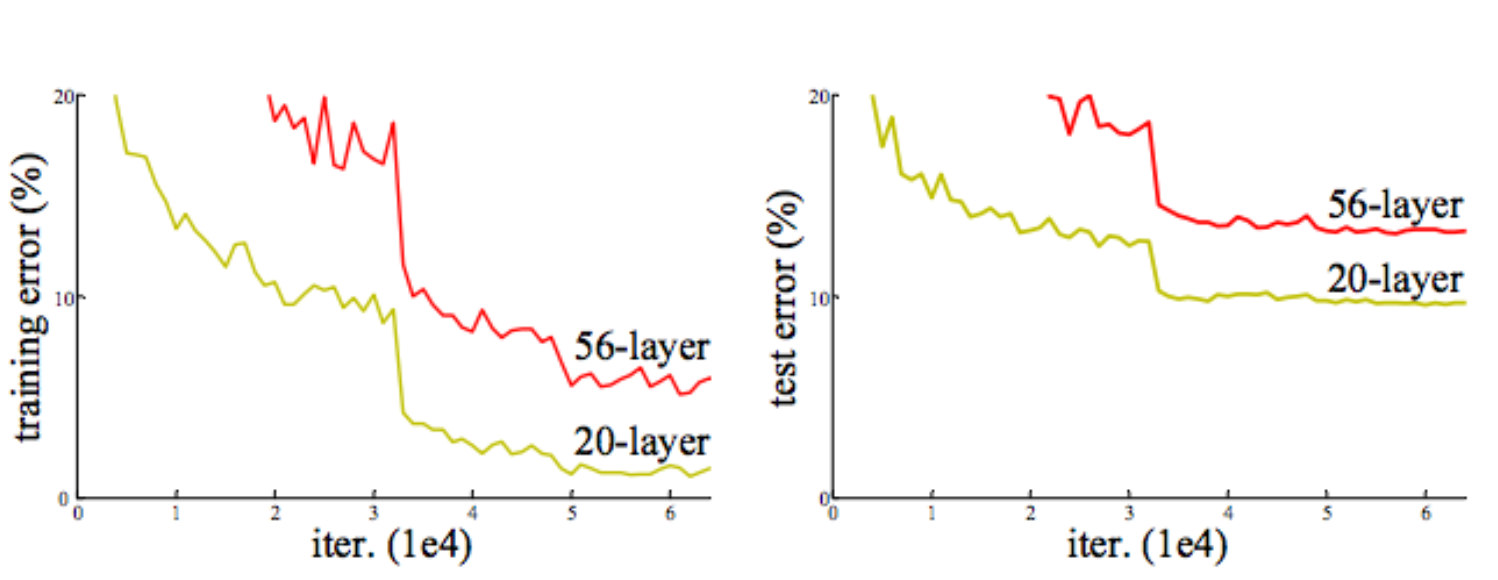
\includegraphics[scale=0.5]{renet1.png}
\end{center}
\caption{An illustration of deep neural networks fails by using the traditional network structure}
 \label{fig:resnet}
 \end{figure}

               
\bibliography{jimmy_shen}
\bibliographystyle{ieeetr}
  
 \end{document}